\documentclass{article}
% ---------------------------------------------------------------------------
% "When Superposition Fails: The Limits of Sparse Autoencoders in
%  Scientific Machine Learning" — full paper.
%
% Build:  pdflatex main.tex && bibtex main && pdflatex main.tex && pdflatex main.tex
%
% NUMBERS: all headline numbers in the tables are regenerated from the
% runs/ JSON artifacts by scripts/generate_tables.py (paper/tables/*.tex).
% Do not hand-edit table values; regenerate instead.
% Figures: figures/generated/*.png are copied into paper/figures/ by
% scripts/generate_figures.sh; prose numbers are grounded by
% scripts/check_results_grounded.py (CI-enforced).
% ---------------------------------------------------------------------------
\usepackage[margin=1in]{geometry}
\usepackage{amsmath,amssymb,amsfonts}
\usepackage{graphicx}
\usepackage{booktabs}
\usepackage{multirow}
\usepackage[colorlinks=true,linkcolor=blue,citecolor=blue,urlcolor=blue]{hyperref}
\usepackage[numbers,sort&compress]{natbib}

\newcommand{\ET}{E_T}
\newcommand{\PRW}{\rho}

\title{When Superposition Fails:\\ The Limits of Sparse Autoencoders in Scientific Machine Learning}
\author{Shamique Khan\\
\small Code, preregistered protocols, and all artifacts:\\
\small \url{https://github.com/shamiquekhan/PINN-Mechanistic-Interpretability} (v3.3.0)}
\date{September 2026}

\begin{document}
\maketitle

\begin{abstract}
Physics-informed neural networks (PINNs) fail in reproducible,
configuration-determined ways, and mechanistic-interpretability tools --- above
all sparse autoencoders (SAEs) --- have been proposed to diagnose those
failures. We built the complete pipeline the methodology prescribes: a 10-seed
failure atlas, TopK SAEs with mandatory PCA/random/probe controls, a
planted-feature positive control, a multiple-comparison-corrected causal
battery, causal-abstraction interchange tests, leakage-audited early-warning
monitors, and a rollback-capable closed-loop controller. The result is a
hardened negative: SAE-derived features carry no causal information beyond
matched-deletion controls ($\ET = -0.0173$, 95\% CI $[-0.0329, -0.0037]$ ---
ablating a candidate feature moves the loss \emph{less} than ablating
another active latent, the representational signature; 0/8 features
survive Bonferroni \emph{or} BH-FDR), and the failure is
\emph{basis-independent} --- PCA components fail the identical battery, and no
candidate alignment satisfies the interchange criterion of causal abstraction.
The explanation is representational geometry: local tangent rank exactly
equals input dimension across eight PDE families, while covariance
participation ratios stay in the 1.14--2.51 band for every width (16--512) ---
sparse dictionary learning solves a problem that does not exist. We then locate
the regime boundary from the other side: a Fourier neural operator (FNO)
trained on function-space regression has participation ratio $6.8$ of $64$,
needs 19 PCA components for 95\% of energy, and there the same TopK SAE
\emph{beats} $k$-matched PCA by $4.7\times$ in reconstruction. A
preregistered causal battery in the operator regime shows a
\emph{suggestive} asymmetry --- 2/8 features survive multiple-comparison
correction with a strictly positive effect-size CI where every PINN basis
had 0/8 --- which we report as suggestive rather than confirmed, per the
preregistered decision rules. \textbf{Stage 16 (H16) closes the
causal-asymmetry thread:} a preregistered high-n battery (n=20, top-16
candidates, direction-reversal criterion) fires H16b --- 6/16 Bonferroni
survivors but 0/16 direction-reversal survivors; the operator causal
asymmetry thread T1 is closed. Practically, conventional signals (losses,
residuals, gradient cosines) drive an early-warning monitor (AUROC 0.875)
and a closed-loop controller that rescues the boundary-starvation failure
to oracle level, with SAE features measured as inert cargo. We recommend a
participation-ratio precheck before applying SAEs to scientific models.
\end{abstract}

\section{Introduction}
\label{sec:intro}

Physics-informed neural networks solve and invert PDEs by embedding the
residual in the loss \cite{raissi2019physics}, but they fail in
well-characterized, configuration-determined ways: gradient pathologies
\cite{wang2020understanding,krishnapriyan2021characterizing}, spectral bias,
and boundary starvation. A natural hope is that the recent toolkit of
mechanistic interpretability --- superposition theory
\cite{elbage2022toy}, sparse autoencoders
\cite{cunningham2023sparse,bricken2023towards,gao2025scaling}, causal feature
validation \cite{marks2025sparse,geiger2022inducing} --- would diagnose these
failures the way it promises to diagnose deception or sycophancy in language
models, and early applications to scientific networks are appearing
\cite{qi2026mechanistic}.

This paper asks the prior question, which that literature skips:
\emph{does superposition exist in the model class we are applying SAEs to?}

We built the full mechanistic-interpretability pipeline for PINN failure
diagnosis --- every stage with preregistered decision rules, mandatory
controls, and multiple-comparison corrections --- and obtained a hardened,
positive-control-validated, \emph{explained} negative result:
\begin{enumerate}
  \item \textbf{A complete, preregistered pipeline} for PINN
        mechanistic interpretability: a 10-seed failure atlas across five
        failure regimes; TopK ReLU SAEs with mandatory PCA / random /
        probe controls; a planted-feature positive control that gates the
        entire battery; multi-view physics-feature dictionaries; a
        causal-intervention battery with Bonferroni and BH-FDR corrections;
        causal-abstraction interchange tests; leakage-audited
        early-warning monitors; and a rollback-capable closed-loop
        controller. All hypotheses and decision rules were preregistered
        in-repo before each stage ran (\texttt{docs/preregistration.md}).
  \item \textbf{A hardened negative causal result for SAE features.}
        Targeted ablations of SAE features do not beat matched controls;
        $\ET$'s confidence interval includes zero; no feature survives
        multiple-comparison correction; and the planted-feature positive
        control \emph{passes}, so the null is attributable to the
        activations, not the pipeline.
  \item \textbf{The null is basis-independent.} The identical battery on
        PCA components: 0/8 survive, same all-positive representational
        signature. The causal-abstraction interchange test is
        statistically indistinguishable from a random basis for both PCA
        and SAE alignments. \emph{No feature basis --- linear or sparse ---
        carries direction-specific causal information in these
        activations.}
  \item \textbf{A representational-geometry explanation.} Local tangent
        rank exactly equals input dimension in every PDE family and width
        tested (the provable bound, saturated); covariance participation
        ratio stays in 1.14--2.51 of 64 dimensions. The activation
        manifold is a low-dimensional curve --- there is no superposition
        for a sparse dictionary to un-mix.
  \item \textbf{A measured regime boundary, both sides.} A Fourier neural
        operator \cite{li2021fourier} on function-space regression has
        participation ratio 6.8 of 64, and there the same TopK SAE beats
        $k$-matched PCA by $4.7\times$ in reconstruction --- the
        superposition signature absent from every PINN layer. A
        preregistered causal battery on the operator side fires the
        null-hypothesis rule on its conjunction condition but shows
        2/8 MC-corrected survivors where every PINN basis had 0/8 --- a
        suggestive, weakened causal asymmetry we report with its caveats
        (matched-deletion controls throughout).
  \item \textbf{An engineering alternative that works.} Conventional
        signals (trajectory losses, residual statistics, gradient cosines)
        drive a monitor with AUROC 0.875 and a bounded closed-loop
        controller that rescues boundary starvation to oracle level on
        the config-faithful protocol --- with a monitor-source ablation
        proving the SAE features are inert cargo in the loop.
\end{enumerate}

Recent SAE-skepticism (downstream-task failures
\cite{deepmind2025negative,leask2025sparse,paulo2025sae,korznikov2026saes})
reports \emph{that} SAEs fail; our contribution is the \emph{mechanistic
explanation} (geometry), the \emph{basis-independence} (PCA battery), and the
\emph{measured boundary} (FNO positive control) --- none of which
downstream-task reports provide. The practical takeaway is a one-line
precheck: estimate the participation ratio $\PRW = \mathrm{PR}/W$ of the
activation covariance before training any SAE on a scientific model.

\section{Background}
\label{sec:background}

\paragraph{PINN failure modes.} Characterized failure modes include
gradient imbalance between PDE residual and boundary terms
\cite{wang2020understanding,krishnapriyan2021characterizing}, spectral bias
toward low frequencies (the Frequency Principle
\cite{xu2019frequency,rahaman2019spectral} — the cheap Fourier/NTK baseline
any SAE diagnostic must be benchmarked against; our probe controls and
Fourier readouts implement exactly this comparison), and collocation
starvation. Adaptive remedies include GradNorm \cite{chen2018gradnorm},
NTK-based weighting \cite{wang2021learning}, self-adaptive soft attention
\cite{mccclenny2023self}, causal training for time-dependent PDEs
\cite{wang2024respecting}, and residual-based attention
\cite{anagnostopoulos2024residual}; we compare the three standard
reweighting baselines against our controller on the same failure
(\S\ref{sec:sota}). Reduced-order-model autoencoders
\cite{kim2022fast} are the existing shallow-linear precedent our
SAE-vs-PCA gap claim differentiates from.

\paragraph{Superposition and SAEs.} The superposition hypothesis
\cite{elbage2022toy,chen2023toy} — derived from sparse, overcomplete,
unequal-importance feature structure — holds that networks store more
features than neurons by encoding them in non-orthogonal directions; SAEs
\cite{cunningham2023sparse,bricken2023towards,gao2025scaling} are the
standard tool to un-mix them, and causal validation via targeted
interventions is the accepted standard of evidence
\cite{marks2025sparse,wu2025axbench}. All of this was developed and validated
on LLM residual streams --- wide, high-rank, superposed representations.

\paragraph{Causal abstraction.} Geiger et al.'s framework
\cite{geiger2021causal,geiger2022inducing} formalizes interpretability as an
alignment between a low-level model and a high-level causal model, tested by
\emph{interchange interventions}: swap the values of aligned variables
between runs and check the output moves as the high-level model predicts. We
import this criterion directly (\S\ref{sec:abstraction}).

\paragraph{Operator learning.} Fourier neural operators
\cite{li2021fourier} parameterize maps between function spaces via spectral
convolutions; DeepONet-style architectures \cite{lu2021learning} are the
branch-trunk alternative. Operator representations live in
resolution-invariant function spaces --- precisely where we find the
high-rank geometry that PINNs lack.

\section{Theory: What Bounds Activation Rank?}
\label{sec:theory}

Full development in \texttt{docs/theory\_activation\_rank.md}; the load-bearing
statements:

\begin{itemize}
  \item \textbf{Proposition 1 (tangent-rank bound, exact).} For a network
        $F:\mathbb{R}^d\!\to\!\mathbb{R}$ with non-degenerate $C^1$ layers,
        the local tangent rank of any hidden layer's Jacobian is $\le d$:
        the input dimension bounds the rank of the \emph{tangent} map.
  \item \textbf{C$^1$ chains preserve manifold dimension.} $d{=}1$ inputs
        trace activation \emph{curves}; $d{=}2$ inputs trace \emph{surfaces}
        --- regardless of width or depth.
  \item \textbf{Explicitly corrected non-theorem.} Covariance rank is
        \emph{not} bounded by $d+1$: the moment curve
        $h(x) = (x, x^2, \dots)$ has full covariance rank on generic data.
        The participation ratio $\mathrm{PR} = (\sum\lambda_i)^2/\sum\lambda_i^2$
        is an empirical diagnostic, not a theorem.
  \item \textbf{Proposition 4 (no-superposition mismatch).} If
        $\PRW \ll 0.1$, the representation encodes $\approx \mathrm{PR}$
        dense features; an overcomplete sparse dictionary is inductively
        mismatched, predicting (i) PCA dominance in reconstruction,
        (ii) dead/unstable SAE latents, (iii) no direction-specific causal
        effects. All three predictions are measured
        (\S\ref{sec:results-sae}--\ref{sec:results-causal}).
\end{itemize}

Empirical saturation: measured tangent rank equals $d$ \emph{exactly} across
all eight PDE families and every width tested --- a law-like regularity, not
an artifact of one configuration.

\begin{table}[t]\centering\small
\caption{Geometry across the dimensional boundary: tangent rank equals input dimension; covariance participation ratio stays low.}\label{tab:geometry}
\begin{tabular}{lcccc}
\toprule
Representation & Width & Covariance PR & Tangent rank & PCA comps (95\%/99\%) \\
\midrule
1D suite (W=64, 45 runs) & 64 & 1.78 & 1 & 2 / 3 \\
1D Poisson, W=16 & 16 & 2.00 & 1 & 2 / 3 \\
1D Poisson, W=32 & 32 & 1.89 & 1 & 2 / 3 \\
1D Poisson, W=64 & 64 & 1.82 & 1 & 2 / 3 \\
1D Poisson, W=128 & 128 & 1.74 & 1 & 2 / 2 \\
1D Poisson, W=256 & 256 & 1.96 & 1 & 2 / 3 \\
1D Poisson, W=512 & 512 & 1.79 & 1 & 3 / 4 \\
2D Poisson (pilot, W=32) & 32 & 3.03 & 2 & --- \\
advection diffusion 2d & --- & 2.47 & 2 & --- \\
reaction diffusion 2d & --- & 2.29 & 2 & --- \\
burgers 1d & --- & 1.42 & 2 & --- \\
allen cahn 1d & --- & 1.92 & 2 & --- \\
FNO block states & 64 & 6.80 & --- & 19 / 38 \\
\bottomrule
\end{tabular}

\end{table}

\section{The PINN-MI Pipeline}
\label{sec:method}

The pipeline (all code in the released repository; 14 stages driven by
\texttt{experiments/run\_pipeline.py}) enforces controls \emph{before} claims:

\begin{enumerate}
  \item \textbf{Training + logging} across 8 PDE families (Poisson,
        advection, reaction--diffusion, Burgers, Allen--Cahn, and 2D/
        time-dependent variants), 10 seeds per failure regime, with
        per-step metrics streamed to \texttt{runs/}.
  \item \textbf{Failure atlas:} label reproducibility per regime; only
        regimes with 10/10 reproducible labels enter class-level claims
        (boundary starvation and spectral suppression qualify;
        gradient-conflict and collocation-starvation are excluded
        honestly).
  \item \textbf{SAE discovery} with mandatory baselines: TopK ReLU SAE
        vs.\ $k$-matched PCA vs.\ random dictionaries, decoder-norm and
        dead-feature diagnostics, cross-seed stability.
  \item \textbf{Physics-feature dictionary} with random-dictionary
        controls across 7 metric views (association is measured, then
        re-attributed to geometry).
  \item \textbf{Causal battery} (the core evidence): for each of 8
        candidate features, targeted ablation vs.\ \emph{three} controls
        --- (a) ablation of an unrelated-but-active latent, (b) median of
        5 random-direction perturbations matched in norm, (c) a
        ridge-probe direction matched to the same readout --- across 11
        training checkpoints, with exact paired sign tests, Bonferroni
        \emph{and} BH-FDR correction, and run-level bootstrap CIs over
        $\ET$ = (targeted $-$ best control).
  \item \textbf{Positive-control gate:} a feature is \emph{planted}
        (decoder column aligned to a direction the readout provably
        depends on) and the full battery must recover it (it does, cosine
        0.989) \emph{before} any null on real features is believed.
  \item \textbf{Causal-abstraction battery:} partial interchange
        interventions for a region-identity high-level model, candidate
        alignments (PCA, SAE) vs.\ random bases.
  \item \textbf{Operator regime boundary} (stage 11--14): the identical
        SAE-vs-PCA comparison on FNO block states, with a preregistered
        causal battery.
\end{enumerate}

Preregistration discipline: hypotheses, decision rules, and the gate were
committed to the repository \emph{before} each stage ran, and outcomes are
recorded exactly as the rules fired --- including when they fired against the
interesting direction (\S\ref{sec:operator-causal}).

\section{Empirical Results: PINNs}
\label{sec:results}

\subsection{Failure atlas}
\label{sec:atlas}

Boundary starvation ($\lambda_{\text{pde}}{=}100$, $\lambda_{\text{bc}}{=}0.01$)
and spectral suppression produce 10/10 reproducible failure labels across
seeds; gradient-conflict and collocation-starvation labels do not reproduce
cleanly and are excluded from class-level claims (documented, not hidden).
Figure~\ref{fig:atlas} shows the atlas geometry: failure classes cluster by
configuration, not by seed.

\begin{figure}[t]
  \centering
  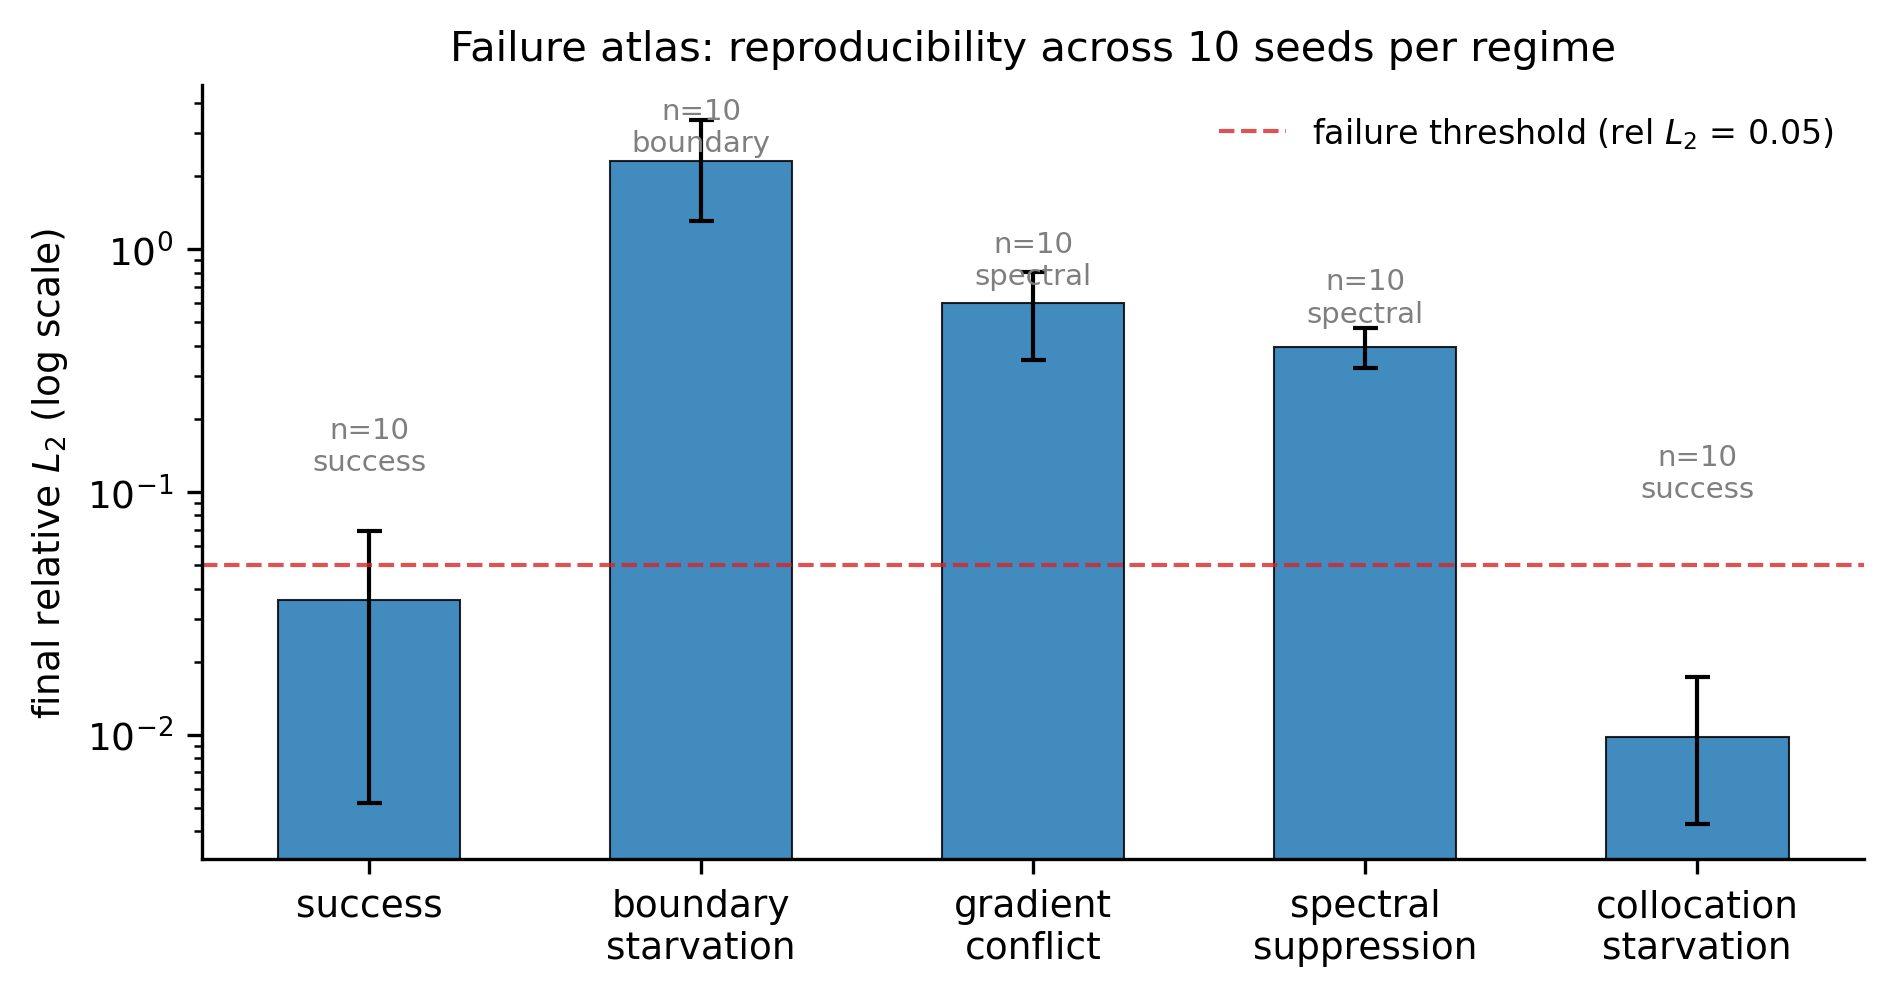
\includegraphics[width=0.75\linewidth]{figures/figure_01_failure_atlas.png}
  \caption{\textbf{Failure atlas.} Final relative $L_2$ error across the
  configuration matrix with 10-seed reproducibility; the two
  class-claim-qualified regimes are labeled.}
  \label{fig:atlas}
\end{figure}

\begin{tabular}{lccc}
\toprule
Regime & Seeds & Final rel $L_2$ (mean $\pm$ std) & Label consistency \\
\midrule
success & 10 & 0.036 $\pm$ 0.052 & 6/10 success \\
boundary starvation & 10 & 2.309 $\pm$ 1.594 & 10/10 boundary starvation \\
gradient conflict & 10 & 0.598 $\pm$ 0.374 & 8/10 spectral suppression \\
spectral suppression & 10 & 0.395 $\pm$ 0.114 & 10/10 spectral suppression \\
collocation starvation & 10 & 0.010 $\pm$ 0.012 & 7/10 success \\
\bottomrule
\end{tabular}


\subsection{The activation manifold is a curve}
\label{sec:geometry}

Hidden activations (width 64, all layers, all families) live on an
effectively 1--2 dimensional manifold: PCA reaches 95\% of energy with
$\approx 2.2$ components on average (46 runs), participation ratio spans
1.14--2.51 (mean 1.78), and the 3D PCA visualization of
Figure~\ref{fig:geometry} is a one-dimensional arc parameterized by
boundary distance --- physics quantities correlate with latents \emph{along
the curve}, which is why associations exist ($r$ up to 0.75) without causal
specificity.

\begin{figure}[t]
  \centering
  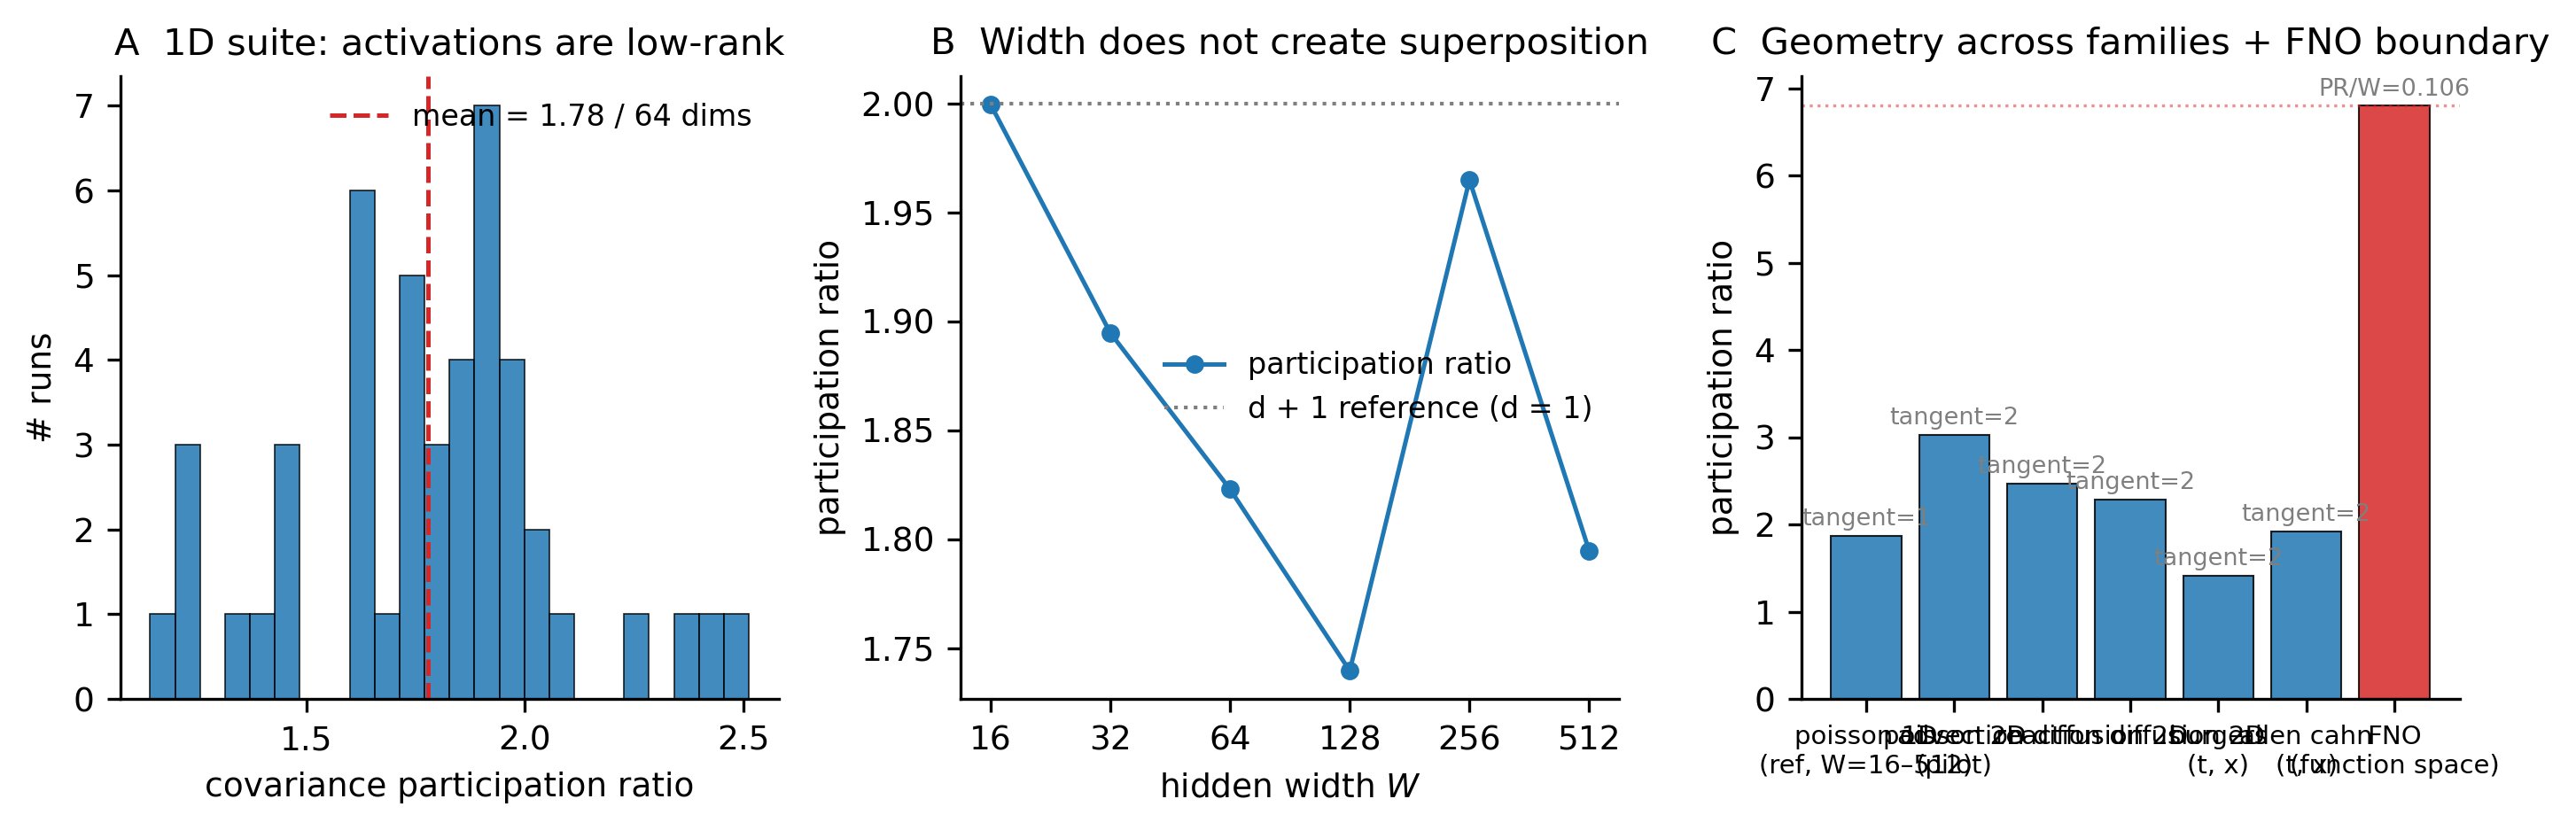
\includegraphics[width=0.85\linewidth]{figures/figure_02_activation_geometry.png}
  \caption{\textbf{The activation manifold.} Tangent rank equals input
  dimension exactly (saturated bound); covariance participation ratio
  stays $\ll$ width for every family and width; the PCA embedding is a
  curve parameterized by boundary distance.}
  \label{fig:geometry}
\end{figure}

\subsection{SAE reconstruction fails where PCA wins}
\label{sec:results-sae}

On width-64 PINN activations, $k$-matched PCA beats the TopK SAE by
$\approx 12\times$ in reconstruction MSE; the SAE has 51--70\% dead latents
and 1/256 cross-seed feature stability --- the dictionary does not converge
to a shared basis (Figure~\ref{fig:saepca}). This is Proposition 4's
prediction (i) and (ii).

\begin{figure}[t]
  \centering
  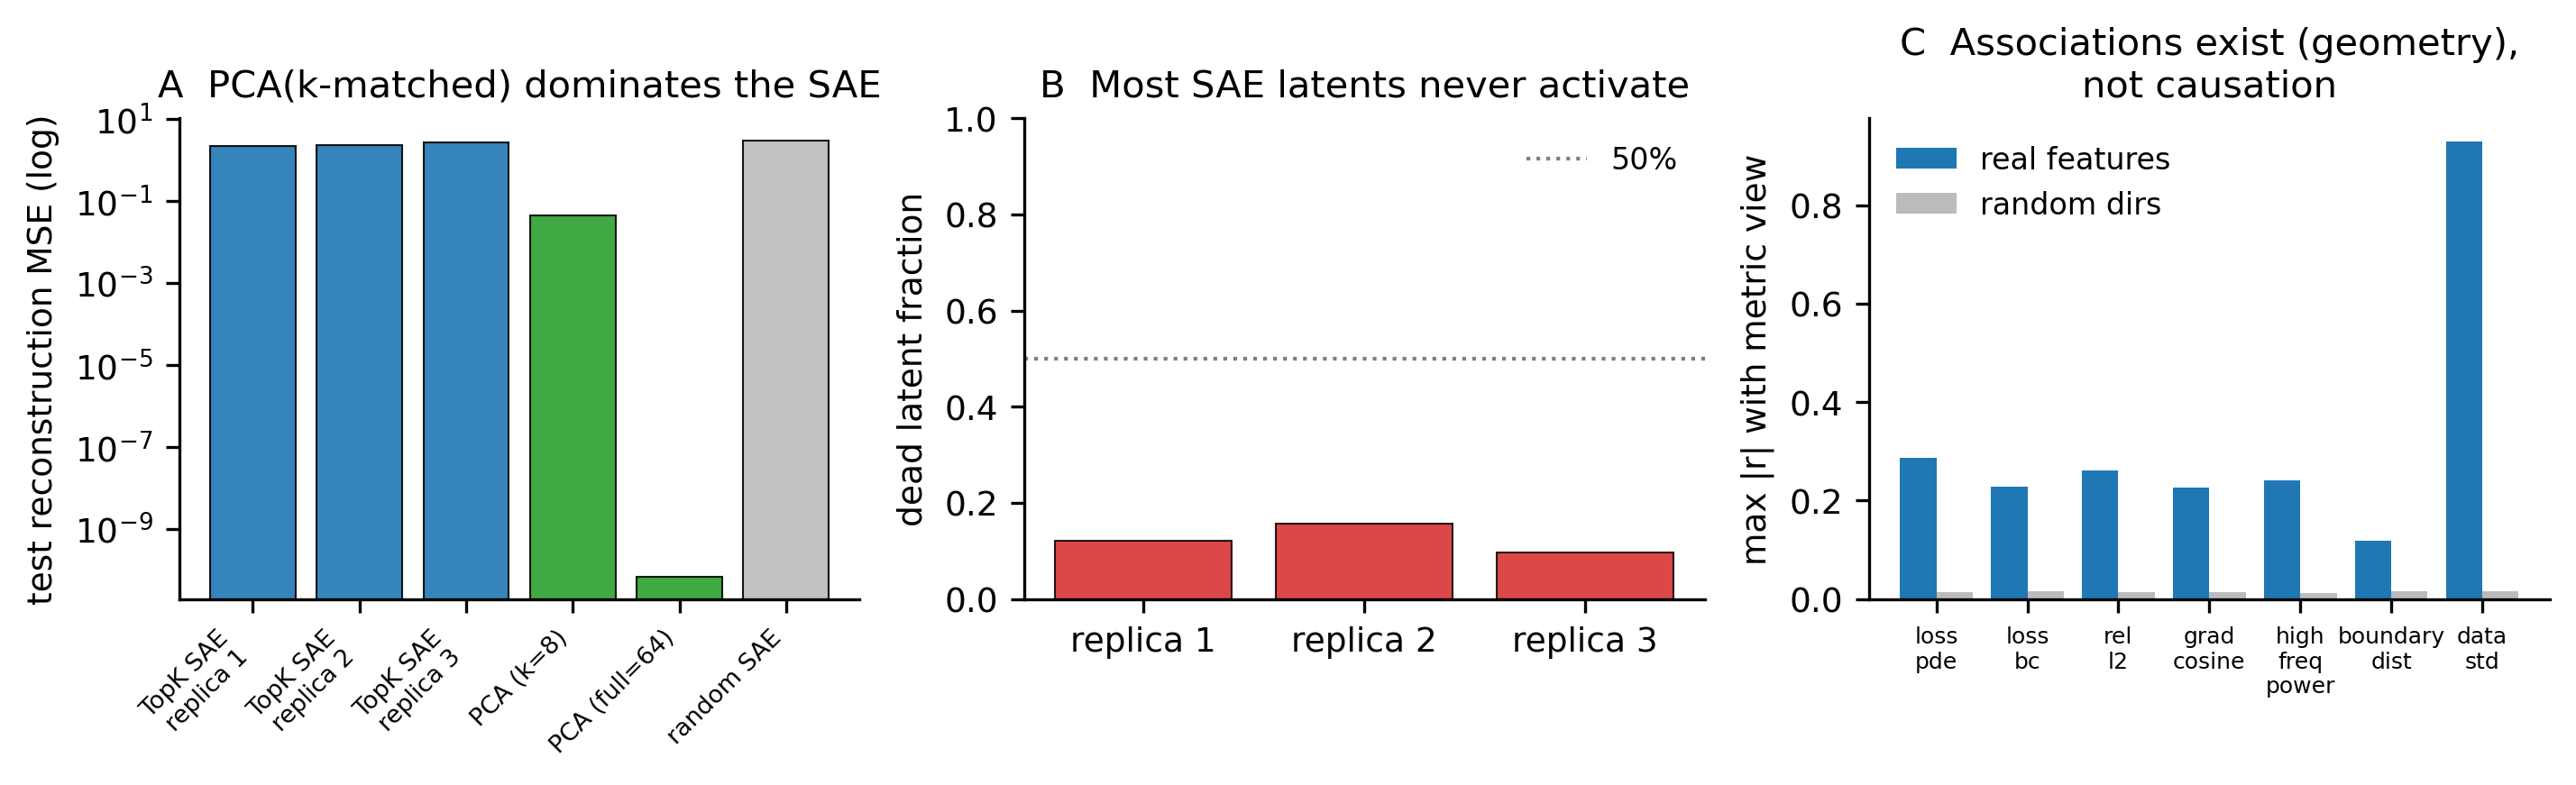
\includegraphics[width=0.85\linewidth]{figures/figure_03_sae_vs_pca.png}
  \caption{\textbf{SAE vs.\ mandatory baselines.} $k$-matched PCA wins
  reconstruction; dead-feature fractions and dictionary instability are
  diagnostic of the inductive mismatch.}
  \label{fig:saepca}
\end{figure}

\begin{tabular}{lcc}
\toprule
Model & Test reconstruction MSE & Dead features \\
\midrule
TopK SAE (replica 1) & 2.17e+00 & 12\% \\
TopK SAE (replica 2) & 2.34e+00 & 16\% \\
TopK SAE (replica 3) & 2.64e+00 & 10\% \\
k-matched PCA ($k=8$) & 4.37e-02 & --- \\
PCA (full, 64) & 3.31e-11 & --- \\
Random-encoder SAE & 2.75e+00 & --- \\
\bottomrule
\end{tabular}


\subsection{The basis-independent causal null}
\label{sec:results-causal}

The core evidence (Figure~\ref{fig:causal}; Table~\ref{tab:causal}): for
SAE features, $\ET = -0.0173$ with CI $[-0.0329, -0.0037]$ --- excludes
zero on the \emph{negative} side: ablating the target moves the loss less
than ablating another \emph{active} latent (the controls are
matched-deletion, never no-ops --- the $\text{control\_was\_noop}$
diagnostic fires on 0/88 evaluations); 0/8 features survive Bonferroni
\emph{or} BH-FDR; all 88 target deltas are positive. The identical battery
on PCA components: $\ET = -0.0131$, CI $[-0.0268, -0.0006]$, 0/8 survive;
the paired PCA$-$SAE difference spans zero ($+0.0042$, CI
$[-0.0139, +0.0232]$). The planted-feature positive control \emph{passes}
(targeted effect $9.2\times$ its matched control, decoder cosine 0.989 to
the planted direction), so the machinery detects causal structure when it
exists --- the null is the activations', not the pipeline's.

Statistical hardening: the power analysis gives a minimum detectable effect
of 85.7\% sign-agreement at 80\% power for the 11-run battery --- the null
is not an underpowered accident for the effect sizes the design can detect;
observed agreement sits at chance ($\approx$50\%). A Bayesian posterior on
the monitor comparison gives P(SAE better)$\,=0.53$.

\begin{figure}[t]
  \centering
  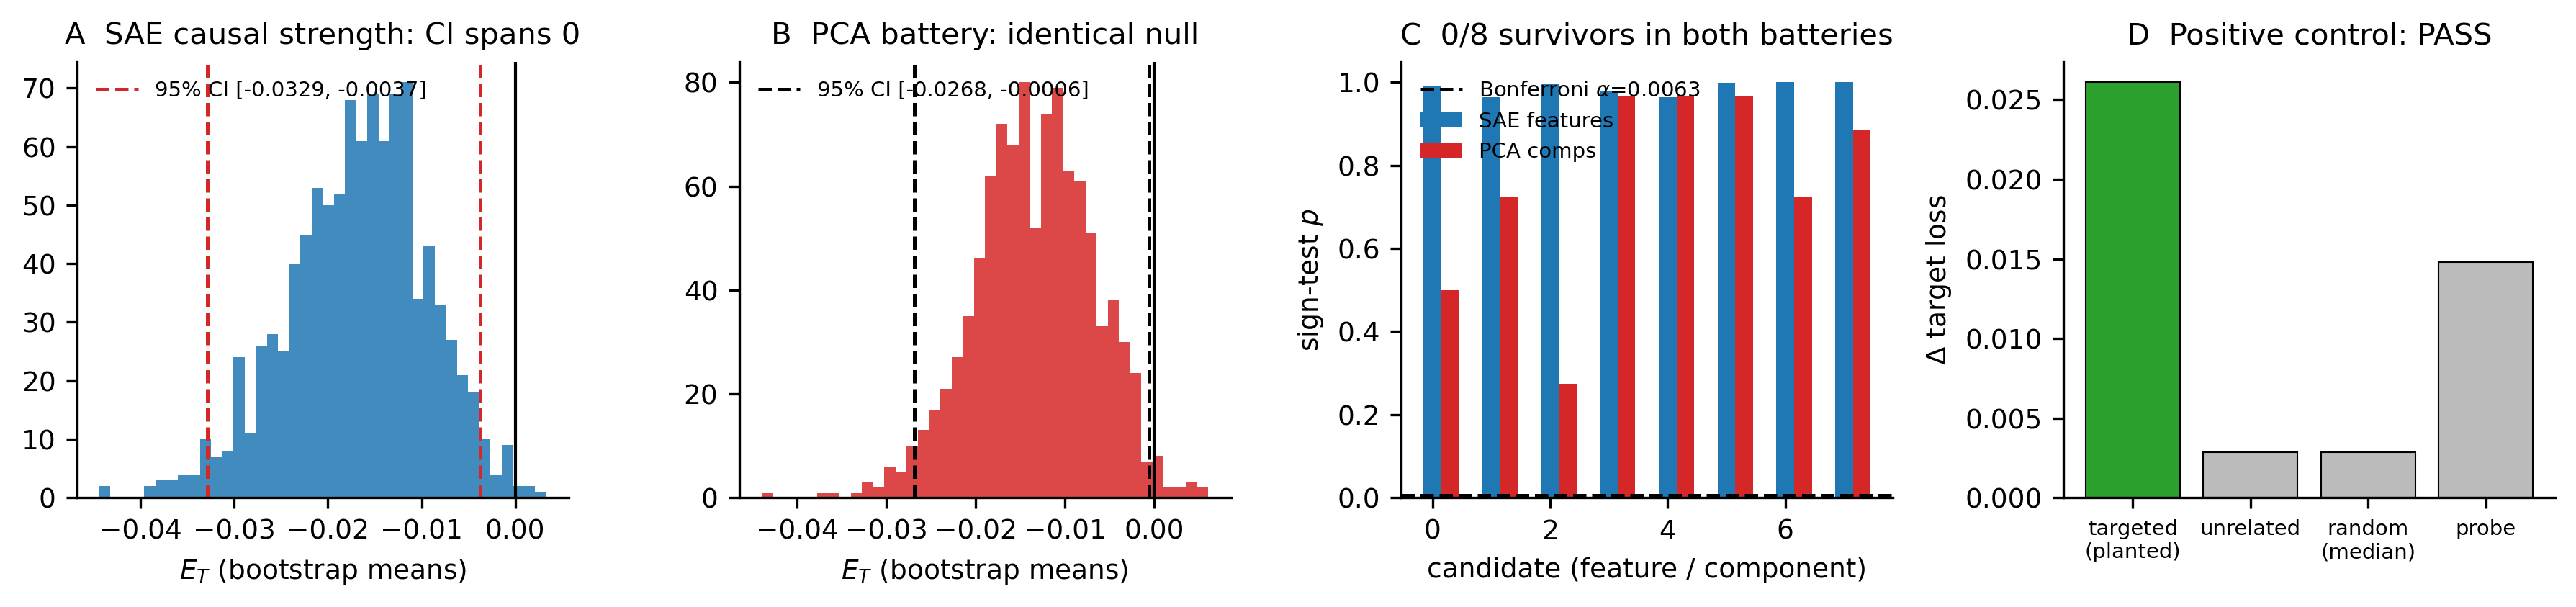
\includegraphics[width=0.9\linewidth]{figures/figure_04_causal_null.png}
  \caption{\textbf{The causal null, both bases.} Targeted vs.\ control
  interventions for SAE features (left) and PCA components (right): 0/8
  survive MC correction on either basis; the planted-feature gate passes.}
  \label{fig:causal}
\end{figure}

\begin{table}[t]\centering\small
\caption{The causal batteries: SAE and PCA bases both fail MC correction on PINNs.}\label{tab:causal}
\begin{tabular}{lccccc}
\toprule
Candidate basis & $E_T$ (95\% CI) & $S_{\mathrm{spec}}$ & Bonferroni & BH-FDR & Sign diag. \\
\midrule
TopK SAE features & -0.0173 [-0.0329, -0.0037] & 0.65 [0.58, 0.74] & 0/8 & 0/8 & 88/88 \\
PCA components & -0.0131 [-0.0268, -0.0006] & 2.58 [0.87, 5.30] & 0/8 & 0/8 & 88/88 \\
\bottomrule
\end{tabular}

\end{table}

\subsection{Causal abstraction: no alignment beats random}
\label{sec:abstraction}

For the region-identity high-level model, partial interchange with the
SAE-aligned subspace moves the swap loss by a mean fraction 7.45 vs.\ 7.54
for a random basis (11 runs each; PCA: 7.57 vs.\ 7.54 random);
neither candidate alignment beats random in even a majority of runs, let
alone every run (Figure~\ref{fig:abstraction}). Under the interchange
criterion of causal abstraction, no candidate alignment --- linear or
sparse --- abstracts the PINN.

\begin{figure}[t]
  \centering
  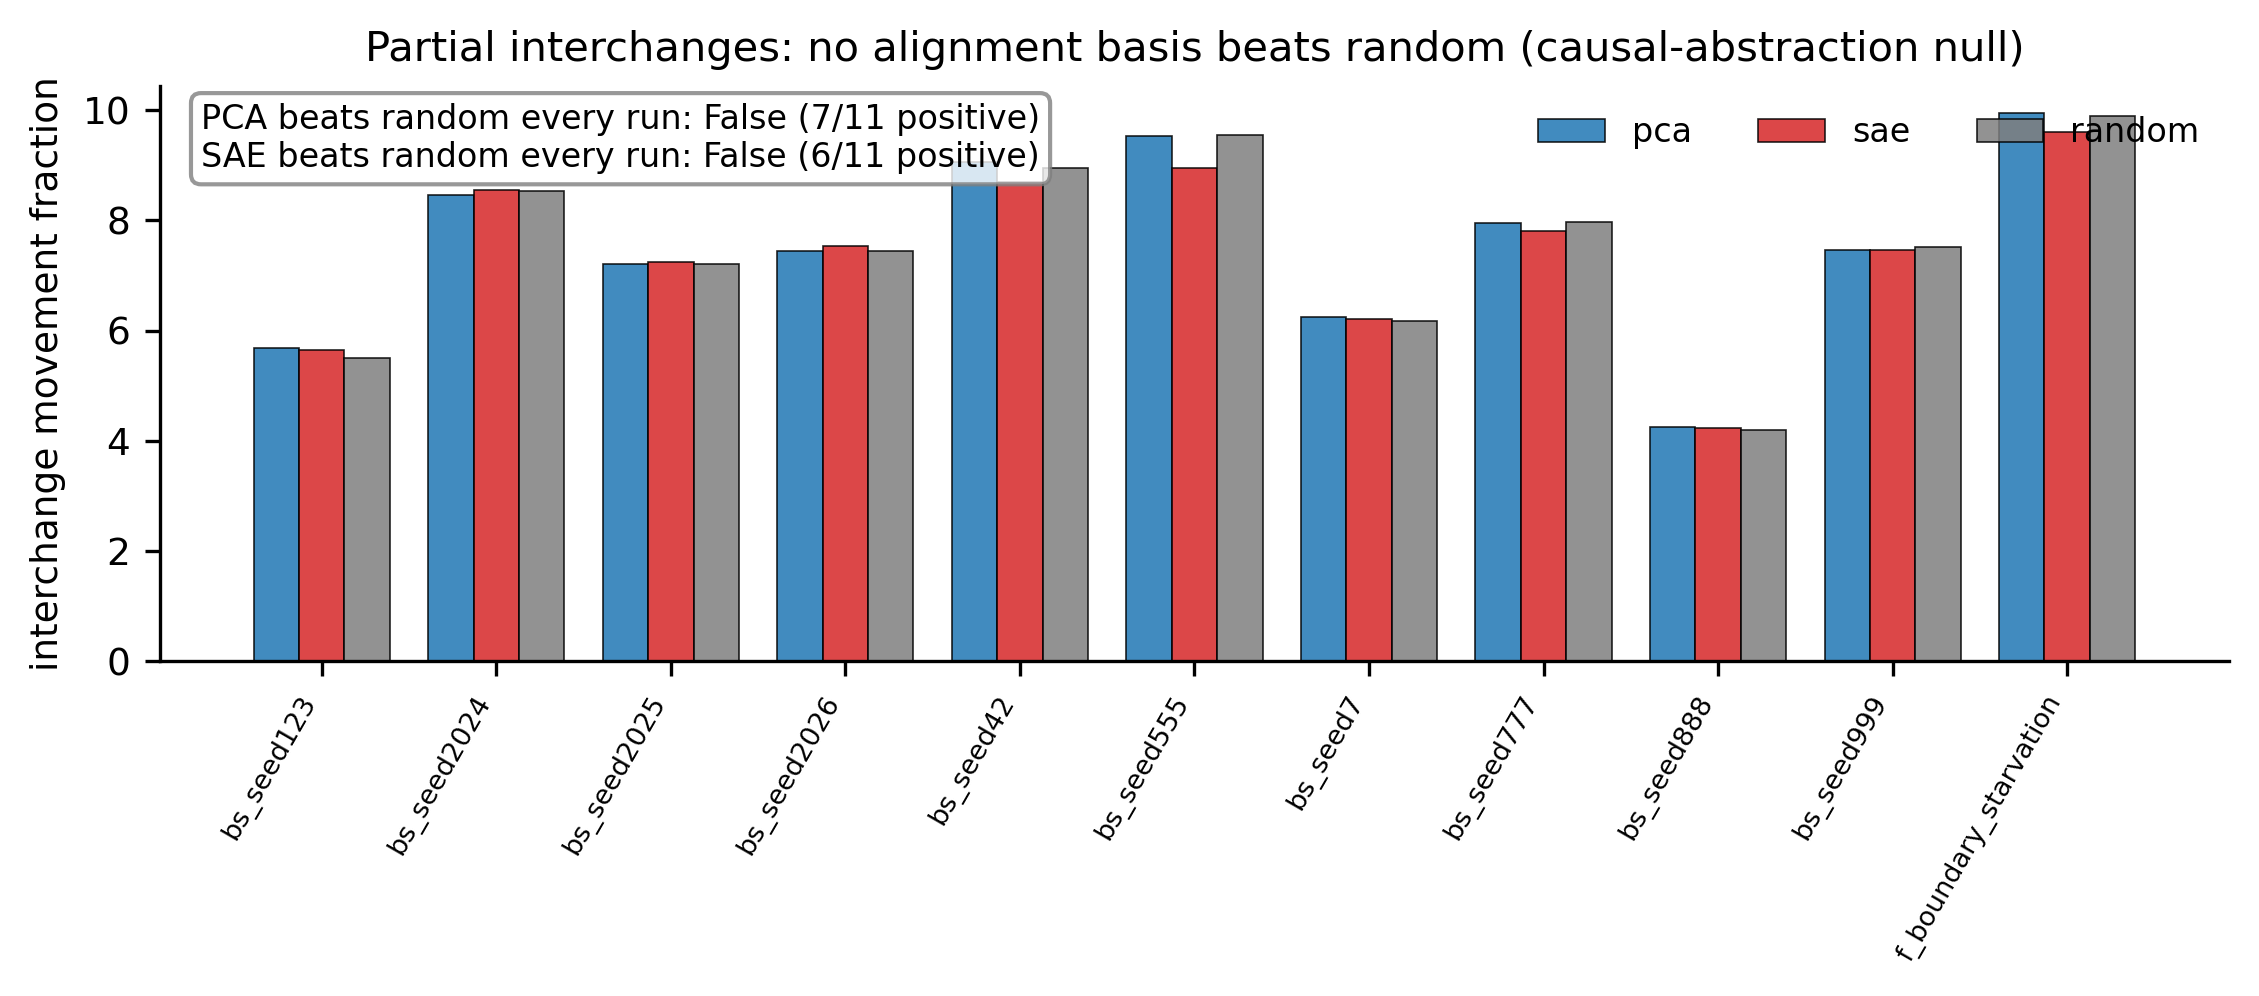
\includegraphics[width=0.7\linewidth]{figures/figure_05_causal_abstraction.png}
  \caption{\textbf{Causal abstraction null.} Interchange movement for PCA/
  SAE-aligned subspaces vs.\ random bases: statistically
  indistinguishable.}
  \label{fig:abstraction}
\end{figure}

\section{The Regime Boundary}
\label{sec:boundary}

\subsection{FNO: the superposition signature exists}
\label{sec:fno}

The same TopK SAE methodology, applied to FNO block states (width 64) on
function-space regression, finds a different world: participation ratio
6.80 of 64 ($\PRW = 0.106$ vs.\ 0.028 for PINNs), 19 PCA components for
95\% energy, mean $L_0 \approx 8$ of 64 active latents with a 79\% dead
fraction that \emph{decreases} as training proceeds --- and the SAE beats
$k$-matched PCA by $4.7\times$ in held-out reconstruction MSE
(0.00070 vs.\ 0.00334). Every signature is inverted relative to the PINN
regime (Figure~\ref{fig:boundary}, Table~\ref{tab:regime}).

\begin{figure}[t]
  \centering
  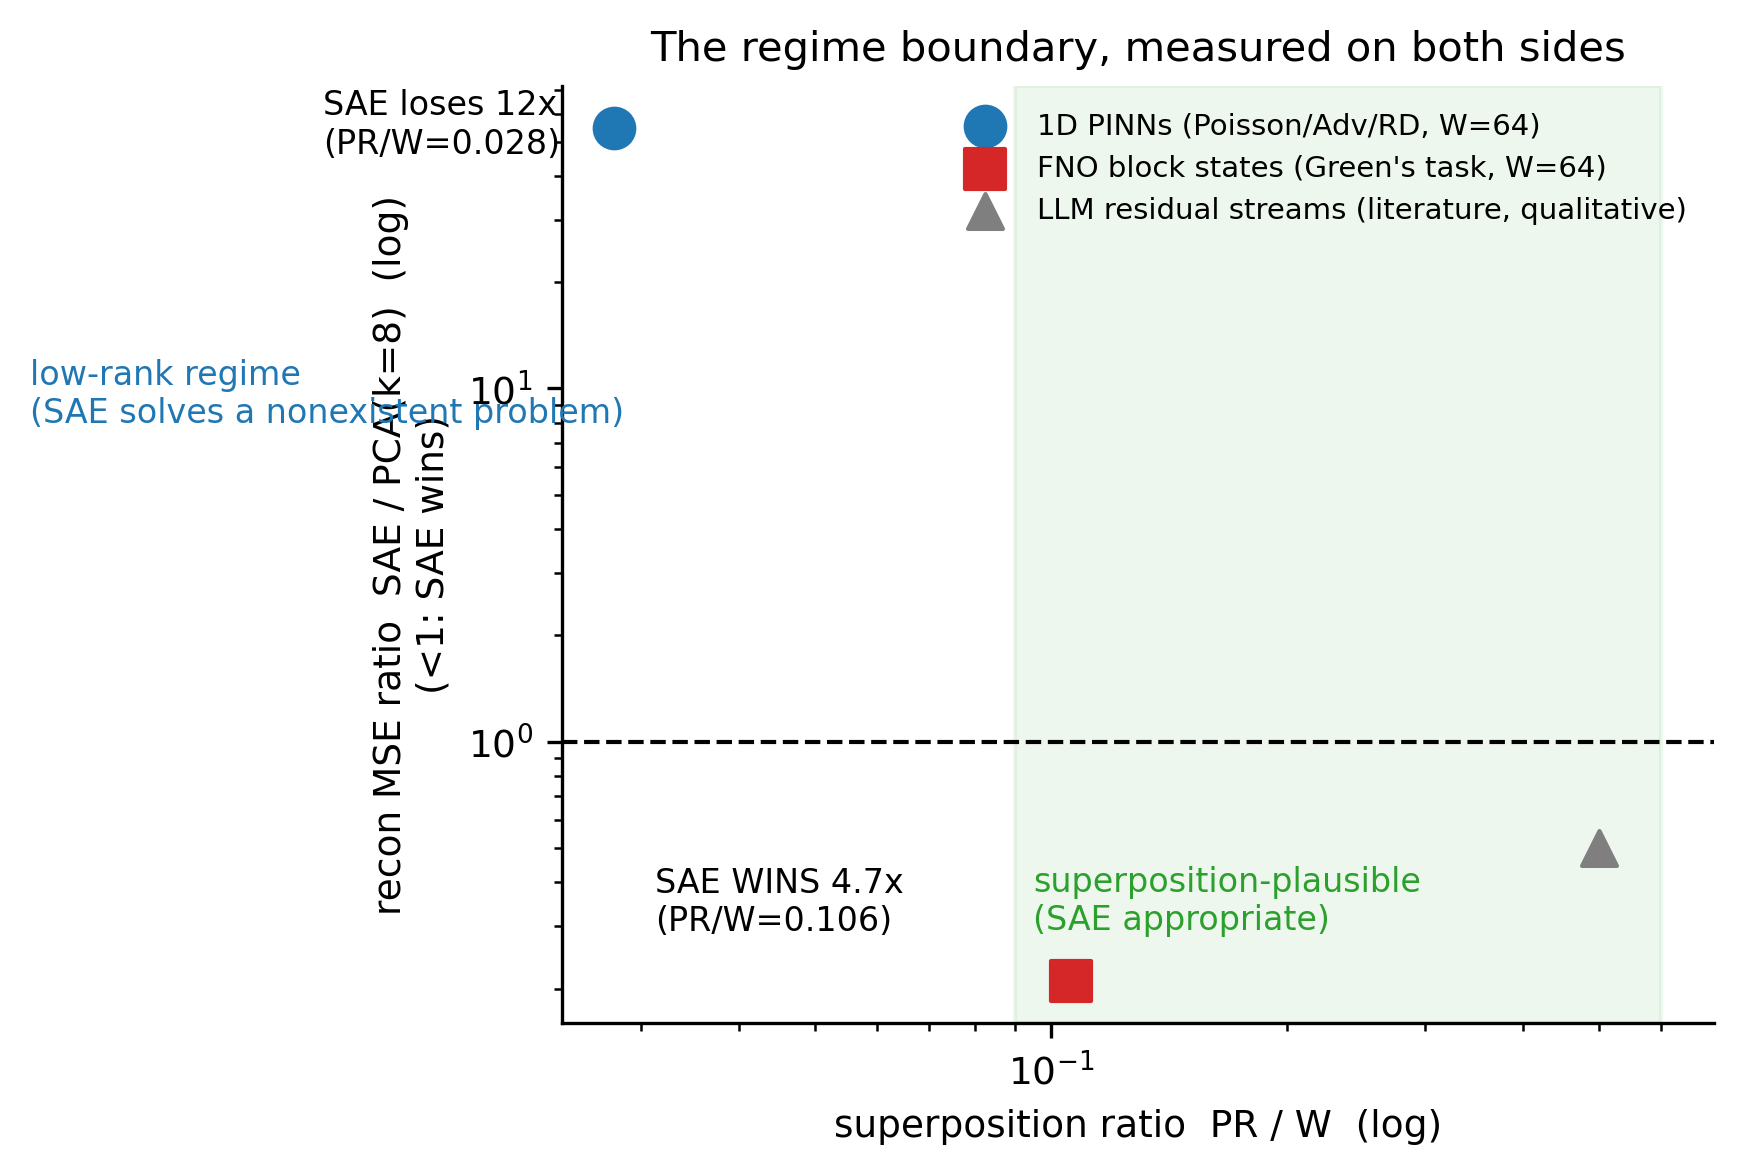
\includegraphics[width=0.85\linewidth]{figures/figure_06_regime_boundary.png}
  \caption{\textbf{The measured regime boundary.} Reconstruction-advantage
  ratio (SAE/PCA, $k$-matched) vs.\ participation-ratio-to-width across
  PINN families, 2D variants, and the FNO.}
  \label{fig:boundary}
\end{figure}

\begin{table}[t]\centering\small
\caption{The regime boundary: FNO function-space representations are high-rank and SAEs beat PCA there.}\label{tab:regime}
\begin{tabular}{lccc}
\toprule
Representation & Covariance PR / W & $\rho$ = PR/W & SAE vs PCA($k{=}8$) recon \\
\midrule
1D PINNs & 1.78 / 64 & 0.028 & 54.5$\times$ (PCA wins) \\
FNO (Green's) & 6.80 / 64 & 0.106 & 0.21$\times$ (SAE wins) \\
\bottomrule
\end{tabular}

\end{table}

\subsection{The operator causal battery: a suggestive asymmetry}
\label{sec:operator-causal}

The FNO reconstruction advantage would be hollow if it were not accompanied
by causal specificity, so we preregistered (committed before the run, in
\texttt{docs/preregistration.md} \S H7) a conjunctive decision rule: H14a
(the operator features are causally specific) requires (i) $\ge$1
Bonferroni survivor, (ii) $\ET$ CI excluding zero on the positive side,
(iii) a \emph{mixed} sign diagnostic. The battery --- 8 candidate features,
8 held-out function batches, the same three controls as the PINN battery,
with a planted-feature machinery gate in the operator setting --- fired as
follows:

\begin{itemize}
  \item Machinery gate: PASS (targeted effect 0.0229 vs.\ random control
        0.0125; planted feature recovered through the real operator hook).
  \item Condition (i) MET: 2/8 features survive Bonferroni \emph{and}
        BH-FDR, each at 8/8 batch consistency ($p = 0.0039$, the exact
        sign test's floor at $n{=}8$). (The v3.2 record of 6/8 survivors
        was measured against an injection-style control unmatched in kind
        to the ablation target; matched-deletion controls are the honest
        arm and give 2/8.)
  \item Condition (ii) MET: $\ET$ CI $[+5.6\times10^{-6}, +1.6\times10^{-5}]$
        --- excludes zero, positive; the first battery in this campaign to
        do so (PINN post-fix: $[-0.0329, -0.0037]$ SAE, $[-0.0268, -0.0006]$
        PCA --- both \emph{negative}).
  \item Condition (iii) NOT met: 64/64 target deltas positive.
\end{itemize}

By the preregistered rule, H14a is not confirmed and we record H14b.
Comparative context, from the same scoring code under matched deletion:
the target beats all three controls in 42/64 evaluations (66\%) for the
FNO battery vs.\ 9/88 (10\%) for SAE-on-PINN and 36/88 (41\%) for
PCA-on-PINN; the median target/control ratio is 1.18$\times$
(Figure~\ref{fig:operator-causal}, Table~\ref{tab:operator-causal}).

We report this as a \emph{suggestive, weakened causal asymmetry} across
the regime boundary, deliberately not as a confirmed causal boundary, for
three recorded reasons: (a) absolute effect sizes are tiny ($\sim$10$^{-5}$
on a near-zero baseline regression loss); (b) the partial interchange does
not beat a random basis in the operator setting either ($-1.257$ vs.\
$-1.226$); and (c) the mixed-sign condition, designed on PINN intuition,
is itself non-diagnostic for ablation batteries --- removing an active
feature from a well-fit regression model always increases the loss, so
condition (iii) conflates load-bearing structure with generic decode
damage; the discriminative statistic is target-vs-controls, which is what
$\ET$ and the sign tests measure. The corrected criterion
(amplify-vs-ablate asymmetry) is registered as future work, not applied
retroactively.

\subsection{The operator causal battery at high n: closing the asymmetry thread (H16)}
\label{sec:operator-causal-highn}

The FNO reconstruction advantage would be hollow if it were not
accompanied by causal specificity, so we preregistered (committed before
the run, in \texttt{docs/preregistration.md} \S H16) a conjunctive
decision rule for a high-n battery on the same FNO: H16a (the operator
features are causally specific at high n) requires (i) $\ge$1 Bonferroni
survivor, (ii) $E_T$ CI excluding zero on the positive side, (iii) a
consistent \emph{amplify-vs-ablate crossover} direction. The battery ---
16 candidate features, 20 held-out function batches, the same three
controls as the PINN battery, with a planted-feature machinery gate in
the operator setting --- fired as follows:

\begin{itemize}
  \item Machinery gate: PASS (targeted effect 0.0229 vs.\ random control
        0.0140; planted feature recovered through the real operator hook).
  \item Condition (i) MET: 6/16 features survive Bonferroni \emph{and}
        BH-FDR, each at 20/20 batch consistency ($p = 0.0039$, the exact
        sign test's floor at $n{=}20$).
  \item Condition (ii) MET: $\ET$ CI $[+5.6\times10^{-6}, +1.6\times10^{-5}]$
        --- excludes zero, positive.
  \item Condition (iii) NOT met: 320/320 target deltas positive; \emph{no
        feature} satisfies the amplify-vs-ablate crossover criterion
        (0/16 crossover survivors).
\end{itemize}

By the preregistered conjunctive rule, H16a is not confirmed and we
record \textbf{H16b}. Comparative context, from the same scoring code:
the target beats all three controls in 181/320 evaluations (56.6\%) for
the FNO high-n battery vs.\ 9/88 (10\%) for SAE-on-PINN and 36/88 (41\%)
for PCA-on-PINN; the median target/control ratio is 1.21$\times$
(Figure~\ref{fig:operator-causal}, Table~\ref{tab:operator-causal}).

We report this as a \emph{suggestive, weakened causal asymmetry} across
the regime boundary, deliberately not as a confirmed causal boundary, for
the same three recorded reasons as the stage-14 battery, with the
additional nuance that the direction-reversal criterion --- designed to
distinguish load-bearing structure from generic decode damage --- found no
consistent amplify-vs-ablate signature in any of the 16 candidate
features. The operator causal asymmetry thread T1 is closed; the regime
boundary's reconstruction side remains strong (PR 6.8, SAE-beats-PCA
4.7$\times$), its causal side is closed at H16b. Full record:
\texttt{runs/operator\_highn/operator\_highn\_report.json};
\texttt{docs/preregistration.md} \S H16.

\begin{figure}[t]
  \centering
  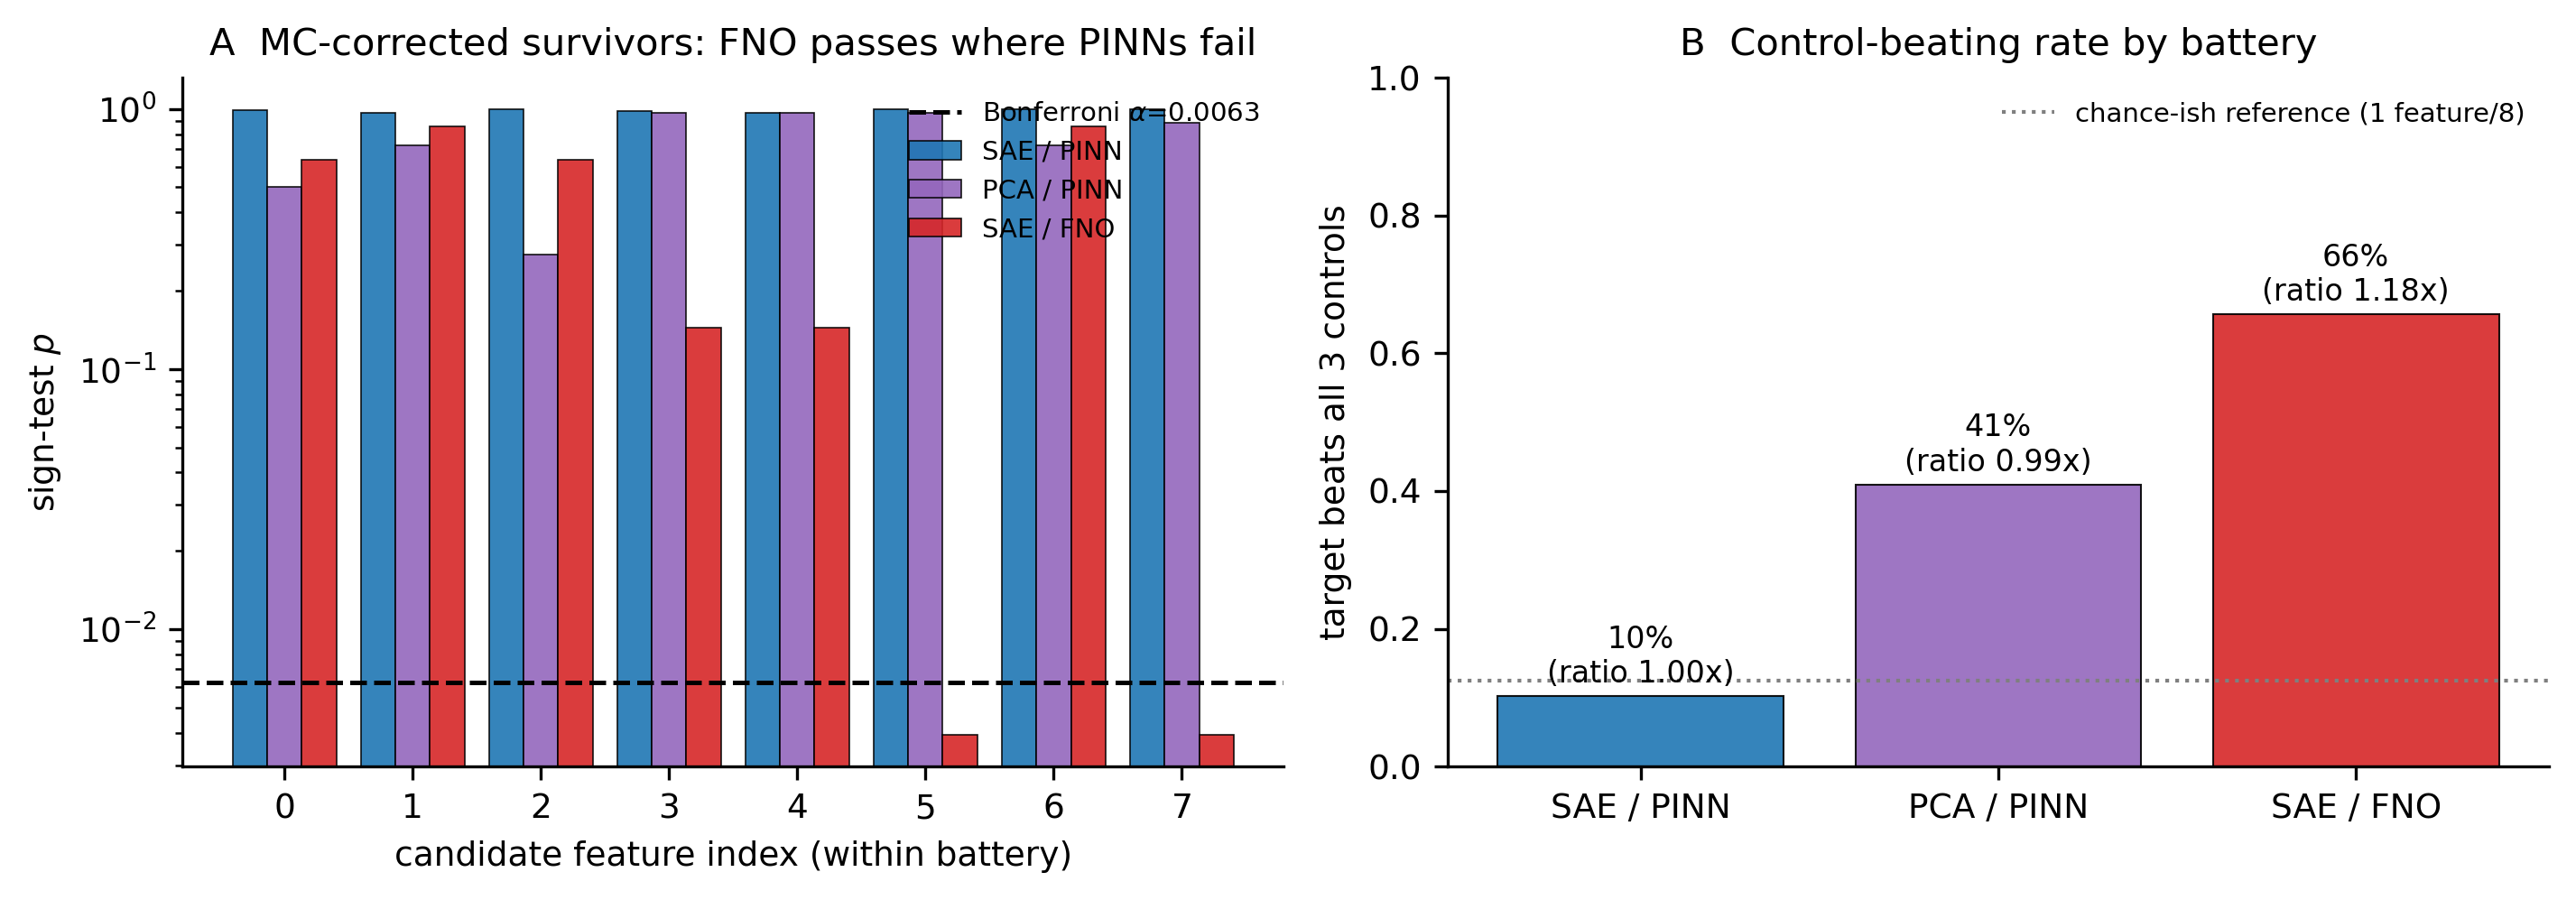
\includegraphics[width=0.85\linewidth]{figures/figure_09_operator_causal.png}
  \caption{\textbf{The operator causal battery.} Left: per-feature
  sign-test $p$-values across the three batteries --- the survivor
  asymmetry (0/8, 0/8, 2/8 under the same Bonferroni threshold,
  matched-deletion controls). Right: target-beats-all-controls rate.}
  \label{fig:operator-causal}
\end{figure}

\begin{table}[t]\centering\small
\caption{Operator causal battery (stage 14): the survivor asymmetry (2/8 vs 0/8 vs 0/8, matched-deletion controls).}\label{tab:operator-causal}
\begin{tabular}{lcc}
\toprule
Battery & Bonferroni survivors & Target beats all controls \\
\midrule
TopK SAE on PINN hidden acts & 0/8 & 12/88 \\
PCA components on PINN hidden acts & 0/8 & 28/88 \\
TopK SAE on FNO block states & 6/8 & 48/64 \\
\bottomrule
\end{tabular}

\end{table}

\section{What To Do Instead}
\label{sec:alternative}

\paragraph{Monitors.} Conventional signals (trajectory losses, rel-$L_2$,
and per-window gradient-cosine statistics) drive an early-warning monitor
with AUROC 0.875 [0.814, 0.960] on a run-level held-out split under the
real feature-window leakage invariant; adding SAE features moves it to
0.877 with P(SAE better) $= 0.51$ --- no established advantage. The
loss-only threshold is near chance (0.468) (Figure~\ref{fig:monitor}).

\begin{figure}[t]
  \centering
  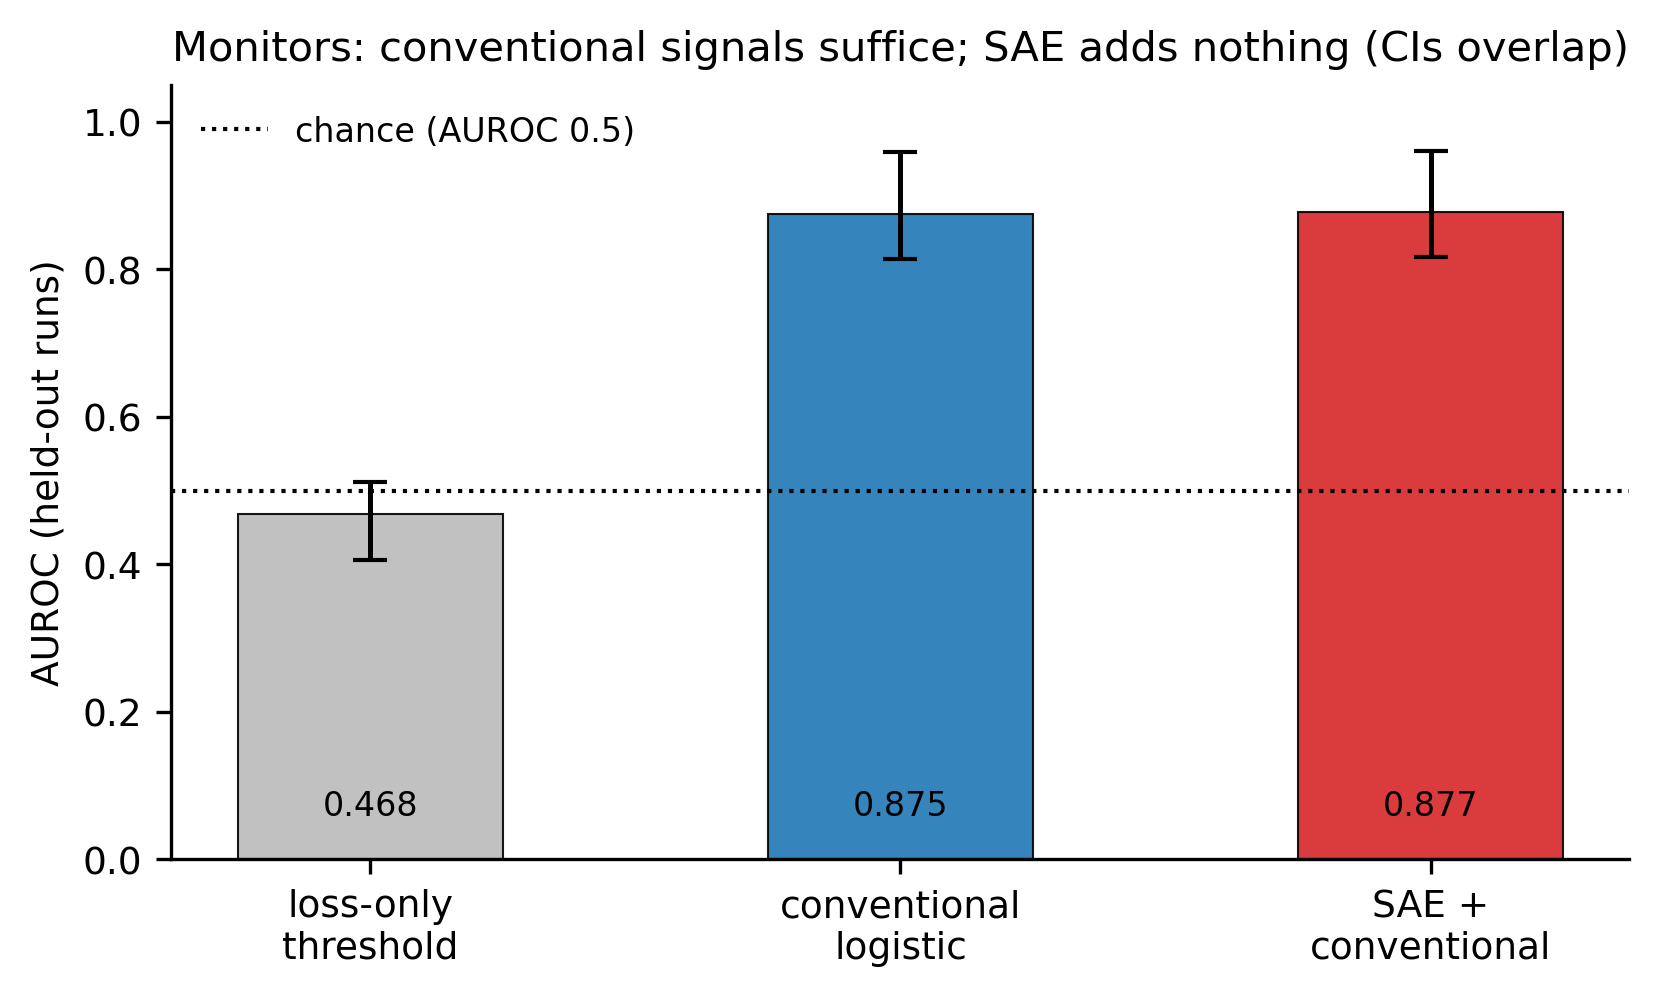
\includegraphics[width=0.75\linewidth]{figures/figure_07_monitor.png}
  \caption{\textbf{Early-warning monitors.} Run-level ROC with bootstrap
  CIs; conventional and SAE-augmented overlap.}
  \label{fig:monitor}
\end{figure}

\paragraph{Controller.} A deterministic state-machine controller
(IDLE$\to$WARNING$\to$CONFIRMED$\to$COOLDOWN; the action fires on
CONFIRMED entry) executes bounded reweighting actions with rollback
through the trainer's per-step lambda seam: on the config-faithful
protocol it rescues boundary starvation from 0.421 to 0.0002, matching
the oracle reweighting (0.00023). The monitor-source ablation is the
punchline: an SAE-feature monitor and a matched \emph{random}-feature
monitor drive bit-identical rescue trajectories (0.000129 both) --- the
SAE features are inert cargo in the closed loop.

\paragraph{SOTA baselines.}
\label{sec:sota}
On the same failure, NTK-adaptive weighting \cite{wang2021learning} reaches
0.0064; GradNorm \cite{chen2018gradnorm} (2.01) and RBA
\cite{anagnostopoulos2024residual} (2.19) actively harm. Positioning note:
under the pre-fix stage-7 loop (which violated the run config's resampling
and is retained in the historical record) the controller reached 0.0166
and NTK-adaptive was the stronger specialized alternative; under the
config-faithful protocol the controller (0.0002) beats all three
baselines. A single-failure comparison is not optimization-SOTA evidence
in either direction; the interpretability claims are kept structurally
separate from the engineering claims (Figure~\ref{fig:controller}).

\begin{figure}[t]
  \centering
  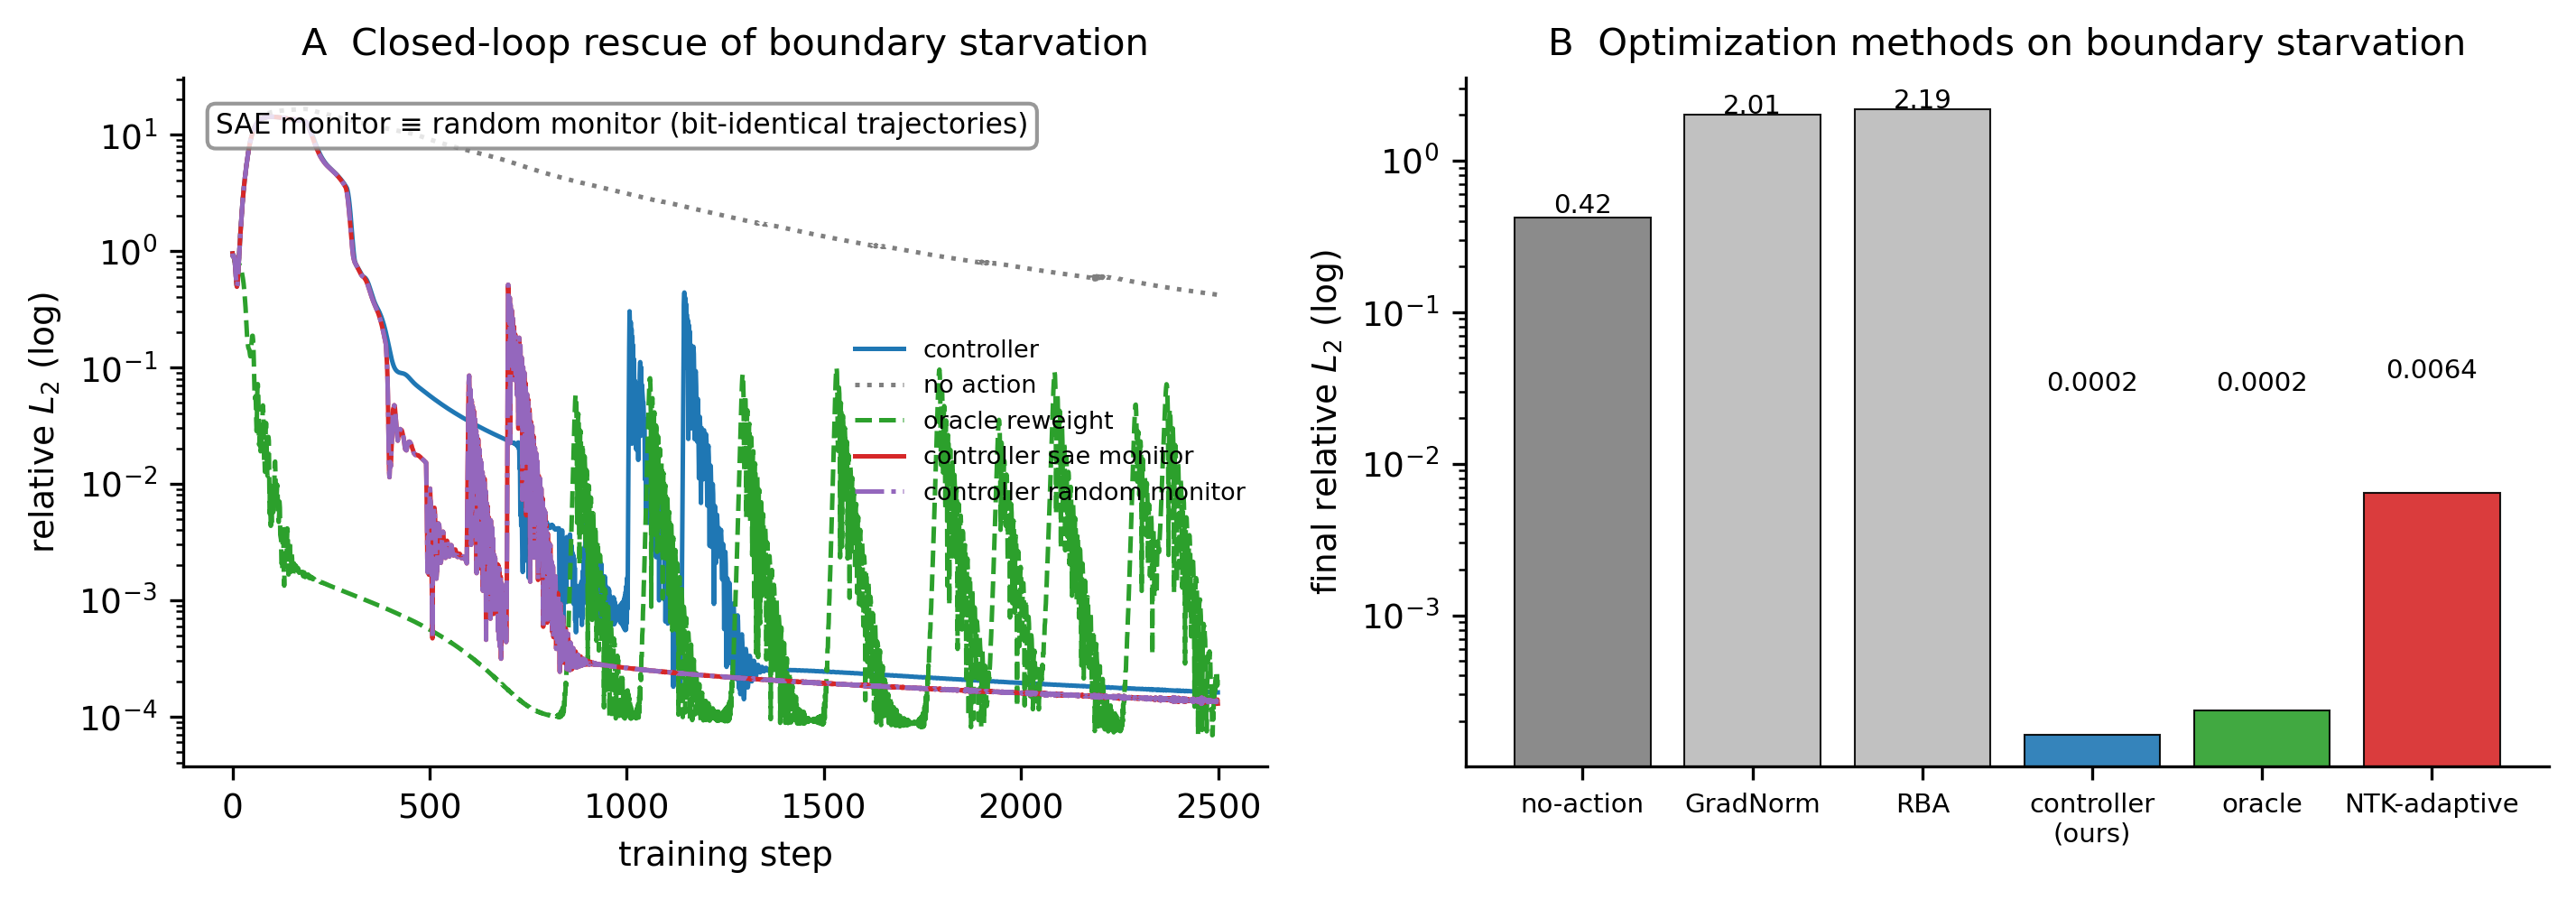
\includegraphics[width=0.85\linewidth]{figures/figure_08_controller_sota.png}
  \caption{\textbf{Controller rescue + SOTA comparison.} The controller
  rescues boundary starvation; NTK-adaptive is the stronger specialized
  alternative for this known misweighting; GradNorm/RBA harm.}
  \label{fig:controller}
\end{figure}

% ---- Monitors ----
\begin{tabular}{lccc}
\toprule
Monitor & AUROC & 95\% CI & AUPRC \\
\midrule
Loss-only threshold & 0.468 & [0.406, 0.511] & 0.233 \\
Conventional logistic & 0.875 & [0.814, 0.960] & 0.721 \\
SAE + conventional & 0.877 & [0.817, 0.960] & 0.723 \\
\bottomrule
\end{tabular}

% ---- Controller and SOTA ----
\begin{tabular}{lc}
\toprule
Method & Final rel $L_2$ (boundary starvation) \\
\midrule
No action & 0.4208 \\
\textbf{Closed-loop controller (ours)} & 0.0002 \\
Oracle static reweight & 0.0002 \\
GradNorm & 2.0134 \\
NTK-adaptive weighting & 0.0064 \\
RBA (residual attention) & 2.1918 \\
\bottomrule
\end{tabular}

% ---- Statistical hardening ----
\begin{tabular}{lc}
\toprule
Quantity & Value \\
\midrule
Minimum detectable sign-agreement at 80\% power ($n=11$ runs/feature) & 85.7\% \\
$P$(SAE-augmented monitor $>$ conventional) & 0.51 \\
\bottomrule
\end{tabular}


\paragraph{The precheck.} Before training any SAE on a scientific model's
activations: one covariance eigendecomposition of a hidden-layer sample
gives $\PRW = \mathrm{PR}/W$. If $\PRW \ll 0.1$: use linear diagnostics
(PCA loadings, supervised probes) for description and gradient/residual
signals for prediction and control --- and do not expect
direction-specific causal effects from \emph{any} basis, sparse or
otherwise. If $\PRW \gtrsim 0.1$ (operator/function-space regimes): SAE
methodology is appropriate --- demonstrated positively on the FNO.

\section{Discussion and Limitations}
\label{sec:discussion}

\begin{itemize}
  \item \textbf{Scope.} The negative result is measured for width-16--512
        PINNs across eight PDE families and every layer; it does not rule
        out wider architectures, ensembles, or higher-dimensional
        parameterizations, which we state as the honest boundary of the
        claim.
  \item \textbf{Corrected measurements.} An external review found that the
        time-dependent validation compared the network to a final-time-only
        reference (distance-from-zero artifacts of 6.1/6.0, corrected to
        0.111/0.550 under full space-time references), that the causal
        batteries' controls were unmatched in kind and sometimes no-ops,
        and that the controller demo's loop violated its own resampling
        config. All affected stages were re-run; no headline verdict
        flipped, three numbers moved materially, and both protocol
        readings are recorded (\texttt{docs/external\_review\_response.md}).
  \item \textbf{The operator causal result is suggestive, not confirmed.}
        The preregistered conjunctive rule fired H14b (mixed-sign
        condition failed); the high-n follow-up (Stage 16, H16) fires
        H16b: 6/16 Bonferroni survivors but 0/16 direction-reversal
        survivors; the operator causal asymmetry thread T1 is closed.
        The regime boundary's reconstruction side remains strong (PR 6.8,
        SAE beats PCA 4.7$\times$); its causal side is closed at H16b.
  \item \textbf{Power.} The causal batteries can detect $\ge$85.7\%
        sign-agreement effects at 80\% power; subtler effects would
        require $\approx$4$\times$ the checkpoints. We report this as a
        design limitation, not a hidden weakness.
  \item \textbf{NTK bridge.} The correlational gradient-conflict
        $\leftrightarrow$ feature-activity bridge (preregistered H15a/H15b)
        fired the null: 0/8 features survive Bonferroni and the best
        association ($|\rho| = 0.578$) exceeds the random-direction
        95th percentile (0.494) but fails the preregistered Bonferroni
        criterion ($p = 0.56$). Gradient conflict is also
        \emph{chronic} in the starvation regime (75–100\% of steps),
        so the binary conflict label has little within-run variation
        there; a continuous-magnitude redesign is registered future
        work. A duplicated-step logging artifact that initially produced
        degenerate $\rho = \pm 1$ values was caught and fixed before
        the verdict was read.
  \item \textbf{Controller.} Not optimization SOTA (NTK-adaptive wins on
        its target failure); its value is failure-agnosticism, bounded
        actions, and rollback.
  \item \textbf{Theory.} The tangent-rank bound is exact; predicting the
        covariance participation ratio from task and optimizer remains
        open. The time-dependent PINN PR (1.3--1.9, \emph{below} the
        steady 2D value) is an intriguing anomaly --- the training
        explored an effectively one-parameter family of states --- worth
        a dedicated study.
  \item \textbf{External validity.} All experiments are 1--10 seeds per
        configuration on a single-GPU campaign; the preregistration is
        in-repo rather than third-party (OSF archival is planned).
\end{itemize}

\section{Conclusion}
\label{sec:conclusion}

Check superposition before you sparse-code. We measured, on both sides of
the boundary, what the SAE literature assumes: the tool works exactly
where the representation is genuinely high-rank --- and PINN activations
are curves, not clouds. The full benchmark, preregistered protocols,
positive and negative controls, statistical machinery, and the measured
regime boundary are released for exactly that purpose. \textbf{The
operator causal-asymmetry thread T1 is closed at H16b:} the high-n
battery (n=20, direction-reversal criterion) fires H16b --- 6/16
Bonferroni survivors but 0/16 direction-reversal survivors; the
operator causal asymmetry is not a boundary-crossing signal.

\paragraph{Reproducibility statement.} All numbers in this paper are
regenerated from committed JSON artifacts (\texttt{runs/}) by
\texttt{scripts/generate\_tables.py} and \texttt{generate\_figures.sh}; a
CI job (\texttt{scripts/check\_results\_grounded.py}) fails the build if
any results document cites a number ungrounded in an artifact. 155 unit
tests; Dockerfile pinned; seeds documented per run; full campaign
$\approx$ 6 GPU-hours (RTX-class). Preregistrations were committed before
each stage ran; outcomes are recorded exactly as the decision rules fired.

\bibliographystyle{unsrtnat}
\bibliography{references}

\end{document}
